\documentclass{beamer}

\setlength{\parskip}{1em}

\title{GRAH-BERT Overview}
\subtitle{Alex To}

%\usetheme{lucid}
\begin{document}
	\frame {
		\titlepage
	}

	\frame{
		\frametitle{Agenda}
		
		\begin{itemize}
			\item Introduction
			\item Linkless Subgraph Batching	
			\item Node Input Vector Embeddings
			\begin{itemize}
				\item Raw Feature Vector Embedding
				\item Weisfeiler Lehman Absolute Role Embedding
				\item Intimacy based Relative Positional Embedding
				\item Hop based Relative Distance Embedding 
			\end{itemize}
			\item Graph Transformer based Encoder
			\item GRAPH-BERT learning
			\begin{itemize}
				\item Pre-training
				\item Model transfer and fine-tuning
			\end{itemize}
		\end{itemize}
	}

	\frame {
		\frametitle{Introduction}
		\begin{itemize}
			\item A graph neural network model
			\item Based on attention mechanism
			\item Train with sampled linkless subgraphs
		\end{itemize}
		\begin{figure}[htb]
			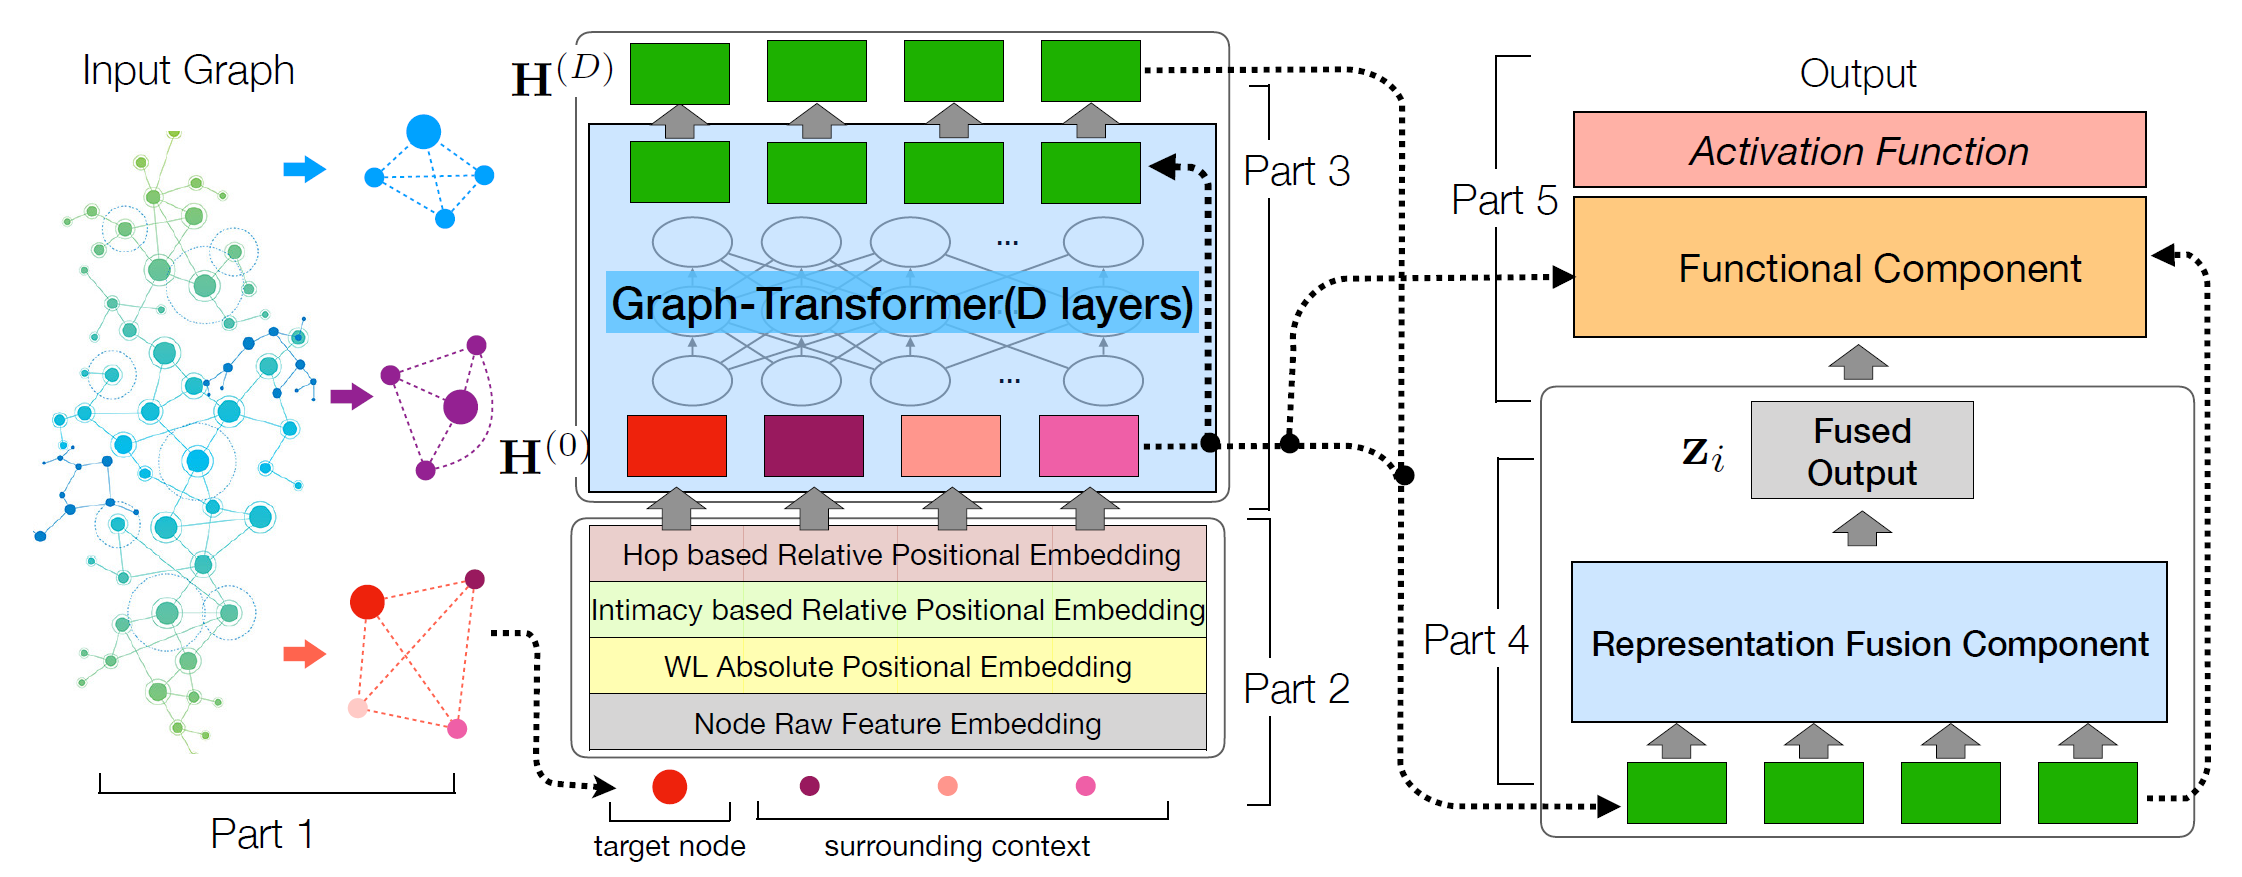
\includegraphics[width=1.0\textwidth]{figures/graph-bert-overview}
			\caption{GRAPH-BERT architecture}
		\end{figure}
	}

	\frame{ 
		\frametitle{Linkless Subgraph Batching}
		Given a graph $G(V,E)$ how to generate sub graph batches?
		
		\begin{itemize}
			\item Calculate an intimacy score matrix $S$
			\[
				S = \alpha \cdot (I - (1 - \alpha) \cdot \bar{A})^{-1}
			\]
			where 
			\[
				\bar{A} = AD^{-1}
			\]
			$A$: adjacency matrix	
			
			$D$: neighbor count diagonal matrix
		
			\item Based on $S$, for a target node $v_i$, find top $k$ "intimate" nodes of $v_i$ with $k$ largest $S(v_i, v_j)$ score.
		\end{itemize}			
	}
	
	\frame {
		\frametitle{Linkless Subgraph Batching (cont)}
		\begin{minipage}{\textwidth}
			\begin{columns}[T,onlytextwidth]
				\begin{column}{.4\textwidth}
					\begin{figure}
						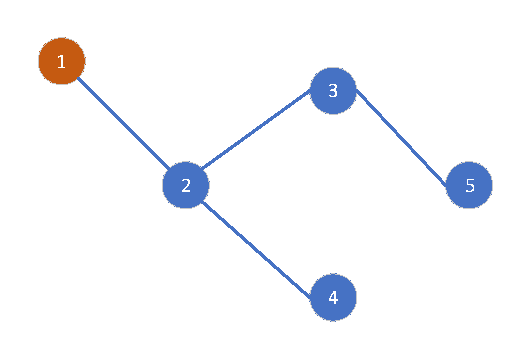
\includegraphics[width=0.9\textwidth]{figures/example-network}
					\end{figure}
				\end{column}
				\begin{column}{.45\textwidth}
					$A = \begin{bmatrix}
					0 & 1 & 0 & 0 & 0 \\
					1 & 0 & 1 & 1 & 0 \\
					0 & 1 & 0 & 0 & 1 \\
					0 & 1 & 0 & 0 & 0 \\
					0 & 0 & 1 & 0 & 0
					\end{bmatrix}$
				\end{column}
			\end{columns}
		\end{minipage}		
	    \begin{onlyenv}<2>
			\begin{minipage}{\textwidth}
				\begin{columns}[T,onlytextwidth]
					\begin{column}{.5\textwidth}
						$D = \begin{bmatrix}
						1 & 0 & 0 & 0 & 0 \\
						0 & 3 & 0 & 0 & 0 \\
						0 & 0 & 2 & 0 & 0 \\
						0 & 0 & 0 & 1 & 0 \\
						0 & 0 & 0 & 0 & 1
						\end{bmatrix}$
					\end{column}
					\begin{column}{.5\textwidth}
						$D^{-1} = \begin{bmatrix}
						1 & 0 & 0 & 0 & 0 \\
						0 & 1/3 & 0 & 0 & 0 \\
						0 & 0 & 1/2 & 0 & 0 \\
						0 & 0 & 0 & 1 & 0 \\
						0 & 0 & 0 & 0 & 1
						\end{bmatrix}$
					\end{column}
				\end{columns}
			\end{minipage}	
		\end{onlyenv}
	}

	\frame {
		\frametitle{Linkless Subgraph Batching (cont)}
		\begin{minipage}{\textwidth}
			$AD^{-1} = \begin{bmatrix}
			0 & 1/3 & 0 & 0 & 0 \\
			1 & 0 & 1/2 & 1 & 0 \\
			0 & 1/3 & 0 & 0 & 1 \\
			0 & 1/3 & 0 & 0 & 0 \\
			0 & 0 & 1/2 & 0 & 0
			\end{bmatrix}$	
		\end{minipage}
		

		
		\begin{minipage}{\textwidth}
			$S = \begin{bmatrix}
			0.259 & 0.128 & 0.085 & 0.109 & 0.072 \\
			0.386 & 0.454 & 0.302 & 0.386 & 0.257 \\
			0.171 & 0.201 & 0.369 & 0.171 & 0.313 \\
			0.109 & 0.128 & 0.085 & 0.259 & 0.072 \\
			0.072 & 0.085 & 0.156 & 0.072 & 0.283 
			\end{bmatrix}$
		\end{minipage}	
	
		For a target node $v_i$, take $k$ entries in $sorted(S(i,:))$, no links (hence, linkless subgraph)
	}

	\frame {
		\frametitle{Node Input Vector Embeddings}
		\begin{figure}
			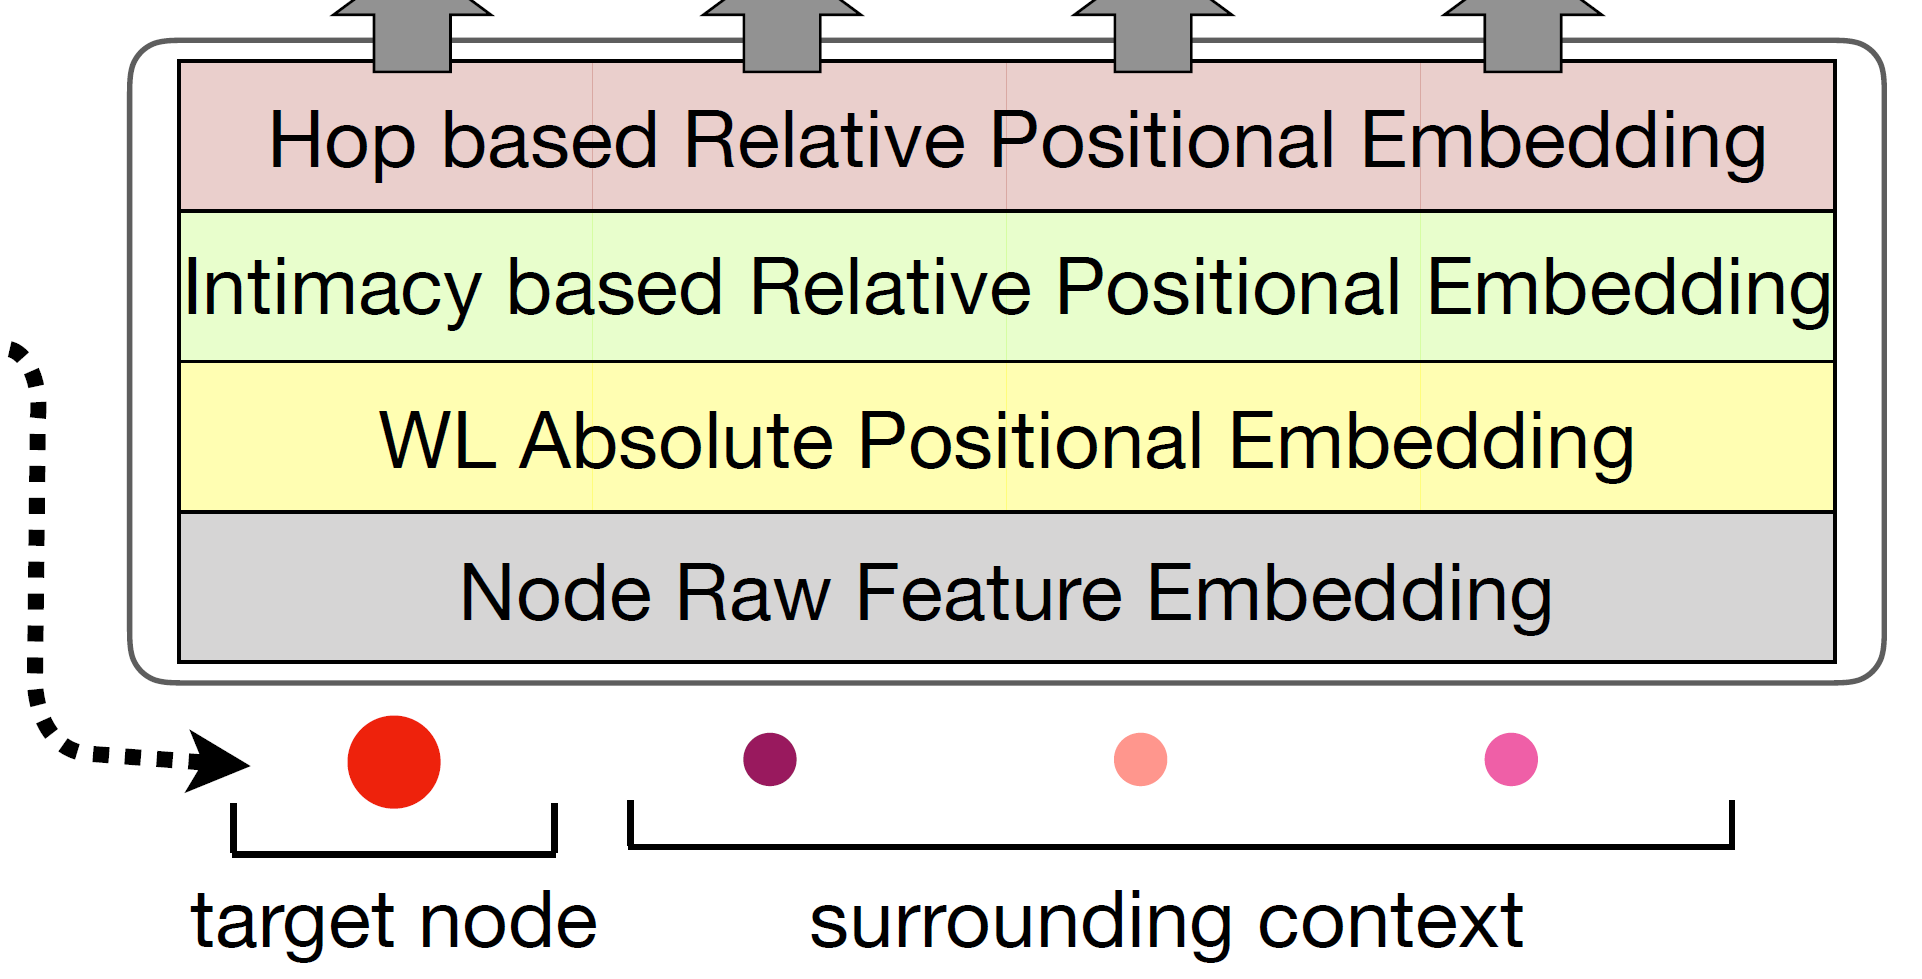
\includegraphics[width=0.7\textwidth]{figures/embeddings}
		\end{figure}
		\begin{itemize}
			\item Raw Feature Vector Embedding
			\item Weisfeiler Lehman Absolute Role Embedding
			\item Intimacy based Relative Positional Embedding
			\item Hop based Relative Distance Embedding 
		\end{itemize}
	}

	\frame {
		\frametitle{Node Input Vector Embeddings}
		\framesubtitle{Raw Feature Vector Embedding}
		
		In each batch, we have
		
		$g_i = \{v_i, v_{i,0}, v_{i,1}, v_{i,2}, ..., v_{i,k}\}$
		
		For each node $v_j \in g_i$
		\[
			e^{(x)}_j = Embed(x_j) \in \mathbb{R}^{d_h}
		\] 
		
		Here $Embed(\cdot)$ function can be CNN if $x_j$ denotes images or LSTM/BERT if $x_j$ denotes texts etc...
		
		=\textgreater each node $v_j$ will be embedded as a vector $\mathbb{R}^{d_h}$
	}
	\frame {
		\frametitle{Node Input Vector Embeddings}
		\framesubtitle{Weisfeiler Lehman Absolute Role Embedding}
		
		
	}
\end{document}